
% Single rooted tree in the form of m_2


\begin{center}
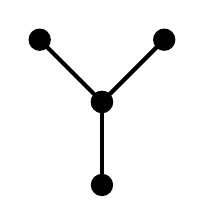
\begin{tikzpicture}[x=0.75pt,y=0.75pt,yscale=-1,xscale=1]
%uncomment if require: \path (0,419); %set diagram left start at 0, and has height of 419

%Straight Lines [id:da8201192265850832] 
\draw [line width=1.5]    (90,60) -- (120,90) ;
\draw [shift={(120,90)}, rotate = 45] [color={rgb, 255:red, 0; green, 0; blue, 0 }  ][fill={rgb, 255:red, 0; green, 0; blue, 0 }  ][line width=1.5]      (0, 0) circle [x radius= 4.36, y radius= 4.36]   ;
\draw [shift={(90,60)}, rotate = 45] [color={rgb, 255:red, 0; green, 0; blue, 0 }  ][fill={rgb, 255:red, 0; green, 0; blue, 0 }  ][line width=1.5]      (0, 0) circle [x radius= 4.36, y radius= 4.36]   ;
%Straight Lines [id:da6726062790054357] 
\draw [line width=1.5]    (120,90) -- (150,60) ;
\draw [shift={(150,60)}, rotate = 315] [color={rgb, 255:red, 0; green, 0; blue, 0 }  ][fill={rgb, 255:red, 0; green, 0; blue, 0 }  ][line width=1.5]      (0, 0) circle [x radius= 4.36, y radius= 4.36]   ;
%Straight Lines [id:da7863057024778404] 
\draw [line width=1.5]    (120,130) -- (120,90) ;
\draw [shift={(120,90)}, rotate = 270] [color={rgb, 255:red, 0; green, 0; blue, 0 }  ][fill={rgb, 255:red, 0; green, 0; blue, 0 }  ][line width=1.5]      (0, 0) circle [x radius= 4.36, y radius= 4.36]   ;
\draw [shift={(120,130)}, rotate = 270] [color={rgb, 255:red, 0; green, 0; blue, 0 }  ][fill={rgb, 255:red, 0; green, 0; blue, 0 }  ][line width=1.5]      (0, 0) circle [x radius= 4.36, y radius= 4.36]   ;
\end{tikzpicture}
\end{center}